\documentclass[11pt]{article}
\usepackage[margin=1in]{geometry}
\usepackage[T1]{fontenc}
\usepackage{lmodern}
\usepackage{microtype}
\usepackage{amsmath,amssymb,amsthm}
\usepackage{booktabs}
\usepackage{graphicx}
\usepackage{xcolor}
\usepackage[numbers,sort]{natbib}
\usepackage[colorlinks=true,linkcolor=blue!50!black,citecolor=blue!50!black,urlcolor=blue!50!black]{hyperref}
\usepackage{caption}
\captionsetup{font=small,labelfont=bf}

\newtheorem{proposition}{Proposition}
\theoremstyle{remark}
\newtheorem{remark}{Remark}
\newcommand{\E}{\mathbb{E}}
\newcommand{\conv}{\operatorname{conv}}
\newcommand{\TV}{\operatorname{TV}}
\newcommand{\todo}[1]{\textcolor{red}{[TODO: #1]}}

\newcommand{\NConfirm}{30}
\newcommand{\NConfirmConflict}{9}
\newcommand{\NConfirmConsensus}{21}
\newcommand{\EOneDiff}{$-$0.029}
\newcommand{\EOneLo}{$-$0.034}
\newcommand{\EOneHi}{$-$0.025}
\newcommand{\EThreeDiff}{$-$0.011}
\newcommand{\EThreeLo}{$-$0.012}
\newcommand{\EThreeHi}{$-$0.009}
\newcommand{\ETwoHarmP}{0}
\newcommand{\ETwoHarmPooled}{7}
\newcommand{\ETwoWorstP}{+0.0056}
\newcommand{\ETwoWorstPooled}{+0.0453}
\newcommand{\ETwoRetain}{90}
\newcommand{\EOneDevDiff}{$-$0.066}
\newcommand{\ConfPrimDelta}{$-$0.230}
\newcommand{\ConfPrimHarm}{0}
\newcommand{\ConfPooledDelta}{$-$0.257}
\newcommand{\ConfPooledHarm}{7}
\newcommand{\ConfMrtsDelta}{$-$0.201}
\newcommand{\ConfMrtsHarm}{0}
\newcommand{\ConfThermoDelta}{$-$0.262}
\newcommand{\ConfThermoHarm}{5}
\newcommand{\ConfThermoGap}{+0.031}
\newcommand{\ConfThermoGapLo}{+0.025}
\newcommand{\ConfThermoGapHi}{+0.037}
\newcommand{\ConfAtsDelta}{$-$0.263}
\newcommand{\ConfAtsHarm}{7}
\newcommand{\ConfAtsGap}{+0.033}
\newcommand{\ConfAtsGapLo}{+0.026}
\newcommand{\ConfAtsGapHi}{+0.039}
\newcommand{\ConfConflictThermoGap}{+0.0002}
\newcommand{\ConfConflictThermoGapLo}{$-$0.005}
\newcommand{\ConfConflictThermoGapHi}{+0.006}
\newcommand{\ConfConflictThermoHarm}{3}
\newcommand{\NLoto}{250}
\newcommand{\NLotoConflict}{75}
\newcommand{\LotoPrimDelta}{$-$0.524}
\newcommand{\LotoPrimHarm}{2}
\newcommand{\LotoPrimWorst}{+0.011}
\newcommand{\LotoPooledDelta}{$-$0.605}
\newcommand{\LotoPooledHarm}{22}
\newcommand{\LotoPooledWorst}{+0.073}
\newcommand{\LotoMrtsDelta}{$-$0.451}
\newcommand{\LotoMrtsHarm}{0}
\newcommand{\LotoMrtsWorst}{+0.001}
\newcommand{\LotoThermoDelta}{$-$0.607}
\newcommand{\LotoThermoHarm}{19}
\newcommand{\LotoThermoWorst}{+0.061}
\newcommand{\LotoAtsDelta}{$-$0.600}
\newcommand{\LotoAtsHarm}{32}
\newcommand{\LotoAtsWorst}{+0.140}
\newcommand{\LotoConstDelta}{$-$0.509}
\newcommand{\LotoConstHarm}{2}
\newcommand{\LotoConstWorst}{+0.013}
\newcommand{\LotoVsMrts}{$-$0.073}
\newcommand{\LotoVsMrtsLo}{$-$0.094}
\newcommand{\LotoVsMrtsHi}{$-$0.054}
\newcommand{\LotoVsMrtsWin}{198}
\newcommand{\LotoVsMrtsLoss}{52}
\newcommand{\LotoVsConst}{$-$0.015}
\newcommand{\LotoVsConstLo}{$-$0.020}
\newcommand{\LotoVsConstHi}{$-$0.011}
\newcommand{\LotoVsConstWin}{161}
\newcommand{\LotoVsConstLoss}{28}
\newcommand{\LotoVsPooled}{+0.080}
\newcommand{\LotoVsPooledLo}{+0.054}
\newcommand{\LotoVsPooledHi}{+0.108}
\newcommand{\LotoVsPooledWin}{61}
\newcommand{\LotoVsPooledLoss}{164}
\newcommand{\LotoRetainLo}{86}
\newcommand{\LotoRetainHi}{87}
\newcommand{\LotoPrimHarmMax}{+0.0108}
\newcommand{\NConflictUnits}{3}

\makeatletter
\newcommand{\inputtable}[1]{\@@input #1 }
\makeatother

\title{Regret-Budgeted Calibration:\\Transferring Temperature Scaling Across Tasks\\While Bounding the Harm to Each Source}
\author{Anonymous authors}
\date{}

\begin{document}
\maketitle

\begin{abstract}
Post-hoc calibrators for the answer probabilities of language models are usually fit on a pool of labelled source tasks and then applied to a new task.
Fitting the pooled likelihood (pooled temperature scaling, Thermometer-style and adaptive-temperature heads) improves the average log-loss on new tasks but makes some of them worse.
The opposite design, minimax-regret temperature scaling (MRTS), never makes a source worse but stays at the identity whenever the sources disagree on the direction of the correction.
For the scalar temperature this is known to follow from a sign test on ``log-loss minus mean entropy'' across sources; we show that for any calibrator class with logits linear in its parameters it happens exactly when the zero vector lies in the convex hull of the per-source loss gradients at the identity.
We propose RB-Cal, which minimises the pooled log-loss subject to a per-source regret budget $\varepsilon$ on a case-clustered upper confidence bound, over a label-free temperature field.
Any $\varepsilon>0$ leaves the identity whenever the pooled loss has a descent direction, and the budget transfers to any target that is a mixture of the sources.
We evaluate five 2025--2026 open-weight instruction models on 31 multiple-choice tasks with a pre-registered protocol and a sealed confirmation split that was scored once.
On the \NConfirm{} sealed target task-units, RB-Cal changes the mean log-loss relative to MRTS by \EOneDiff{} nats (95\% CI [\EOneLo, \EOneHi]) with no harmed unit, keeps \ETwoRetain\% of the pooled gain, and harms \ETwoHarmP{} units where pooled temperature scaling harms \ETwoHarmPooled.
A leave-one-task-out analysis over \NLoto{} target task-units shows the same trade-off: RB-Cal harms \LotoPrimHarm{} units (largest regret \LotoPrimHarmMax{} nats) against \LotoPooledHarm, \LotoThermoHarm{} and \LotoAtsHarm{} for pooled temperature scaling, Thermometer-P and ATS-P, while giving up about \LotoRetainLo--\LotoRetainHi\% of their mean gain.
RB-Cal does not beat the pooled methods on average log-loss; its contribution is the trade-off.
\end{abstract}

\section{Introduction}
Language models used for multiple-choice question answering produce a distribution over the answer options.
These distributions are often miscalibrated~\citep{kadavath2022know,zhao2021calibrate}, and the size and even the direction of the miscalibration change from task to task, from model to model and with the prompt.
The standard remedy is post-hoc temperature scaling~\citep{guo2017calibration,platt1999probabilistic}, which needs labelled data from the task it is applied to.
When a model is deployed on a task without labels, the calibrator has to be learned on other, labelled tasks and transferred~\citep{yu2022multidomain,shen2024thermometer,xie2024ats}.

Transfer creates a safety question that averages hide.
A calibrator fit to the pooled log-loss of many sources moves in the direction that helps most sources and hurts the rest.
In our data, pooled temperature scaling increases the log-loss by more than 0.01 nats on \ConfPooledHarm{} of \NConfirm{} sealed target task-units and on \LotoPooledHarm{} of \NLoto{} held-out source task-units.
Learned input-dependent temperatures (our probability-feature adaptations of Thermometer~\citep{shen2024thermometer} and of adaptive temperature scaling~\citep{xie2024ats}) behave the same way.
A practitioner who calibrates in order to make probabilities more trustworthy will reasonably want a method that rarely makes them worse.

The conservative alternative is to require that no source gets worse.
Minimax-regret temperature scaling (MRTS; \citet{calport2026}) picks the scalar temperature that minimises the largest per-source change in log-loss.
It never hurts a source, but with many sources it frequently returns the identity and does nothing.
\citet{calport2026} prove that this happens as soon as one source is overconfident and another underconfident, which is common with 25 heterogeneous sources (``conflict regime'').
Section~\ref{sec:theory} extends their condition to richer calibrator classes: the identity is minimax-optimal if and only if $0$ lies in the convex hull of the per-source gradients at the identity.

We study the space between these two extremes.
\textbf{RB-Cal} (regret-budgeted calibration) minimises the pooled log-loss subject to a budget $\varepsilon$ on every source's regret, measured relative to the uncalibrated model.
The budget is placed on a case-clustered upper confidence bound of the regret so that noisy sources do not use the whole budget, and the calibrator is a label-free temperature field $\beta(p)$ over entropy, top-1 probability and margin.
Our contributions:
\begin{itemize}
\item \textbf{A diagnosis of when minimax calibration does nothing} for any calibrator class with logits linear in its parameters (Proposition~\ref{prop:stuck}), which contains the scalar sign condition of \citet{calport2026} as a special case, and a converse for the budgeted problem (Proposition~\ref{prop:escape}).
\item \textbf{RB-Cal}, a budgeted convex objective with a statistical (UCB) version of the budget, a source-only selection rule and a deployment gate, together with a transfer statement for targets close to a mixture of sources (Proposition~\ref{prop:transfer}).
\item \textbf{A pre-registered evaluation} on five recent open-weight models, two prompts and 31 tasks, with a development split, a sealed confirmation split scored once after freezing the code, and two secondary analyses run afterwards: two additional baselines and leave-one-task-out over 25 source tasks.
All deviations from the pre-registration are reported (Appendix~\ref{app:protocol}).
\end{itemize}
The results are a trade-off, not a dominance result.
RB-Cal beats MRTS on mean log-loss with no more harm in the sealed split and gives up roughly a tenth of the pooled methods' mean gain in exchange for an order of magnitude fewer harmed task-units.

\section{Related work}
\paragraph{Post-hoc calibration.}
Temperature scaling~\citep{guo2017calibration} and its relatives fit a few parameters on held-out labelled data.
Richer maps include entropy-dependent temperatures~\citep{balanya2024adaptive}, order-preserving functions~\citep{rahimi2020intra}, ensembles of calibrators~\citep{zhang2020mixnmatch} and top-versus-all reformulations~\citep{lecoz2024tva}.
They assume labels from the deployment distribution, which is the assumption we drop.

\paragraph{Calibration under shift and across domains.}
Calibration degrades under dataset shift~\citep{ovadia2019trust}.
Multi-domain temperature scaling~\citep{yu2022multidomain} learns, from several labelled domains, a map from domain features to a temperature, so that an unseen domain receives its own temperature.
Calibration for domain generalisation~\citep{gong2021dgcal} and consistency-guided temperature scaling~\citep{choi2024cts} also learn from several labelled source domains for an unseen one, without target data.
TransCal~\citep{wang2020transcal} uses unlabelled target data for domain adaptation.
For language models, Thermometer~\citep{shen2024thermometer} trains an auxiliary network across tasks that predicts a task temperature from unlabelled inputs, and adaptive temperature scaling (ATS)~\citep{xie2024ats} predicts a temperature for each token from hidden states.
All of these optimise an average over sources; none bounds the loss on individual sources.
\citet{calport2026} audit this risk directly: across typed decision tasks and standard benchmarks, pooled source temperatures often harm new tasks, and they propose MRTS, prove that it returns the identity when two sources disagree in sign, and compare it with a sign-consensus rule, shrinkage and a re-implemented Thermometer.
We take MRTS as the safe end of the spectrum and ask how much of the pooled gain can be recovered while still bounding every source's regret.
Hidden regions of over- and underconfidence in language models have also been studied directly~\citep{kobalczyk2026hidden}.

\paragraph{Worst-group and constrained learning.}
Group DRO~\citep{sagawa2020dro} minimises the worst group loss; MRTS is its calibration analogue with regret instead of loss.
Constrained learning~\citep{chamon2020pac} minimises an average subject to constraints on other losses, and RB-Cal is an instance with one constraint per source.
Placing the constraint on a high-confidence bound of an estimated quantity follows high-confidence policy improvement and Seldonian algorithms~\citep{thomas2015hcpi,thomas2019seldonian}; risk-controlling selection with formal guarantees is studied in Learn-then-Test~\citep{angelopoulos2021ltt}.
Our UCB constraint borrows this idea but does not carry their guarantees (Section~\ref{sec:theory}, Remark~\ref{rem:ucb}).
The common-descent test is the min-norm problem of the multiple-gradient descent algorithm~\citep{desideri2012mgda,sener2018mtl}; conflict between task gradients is the starting point of conflict-averse multi-task optimisation~\citep{liu2021cagrad}.
What is specific here is the use of that geometry as a diagnostic that predicts when source-safe calibration can move at all, and its scalar reduction to an entropy--log-loss sign test.
The mixture assumption in Proposition~\ref{prop:transfer} is the one of multiple-source domain adaptation~\citep{mansour2009multiple}.

\section{Setup}\label{sec:setup}
A \emph{unit} is a model--prompt pair; every unit gets its own calibrator.
For a question with $K$ options the unit outputs probabilities $p\in\Delta^{K-1}$, floored at $10^{-12}$ and renormalised.
A calibrator maps $p$ to $q_\theta(\cdot\mid p)$; the identity $\theta_0$ returns $q=p$.
Each labelled source task $w\in\{1,\dots,W\}$ has a distribution $D_w$ over $(p,y)$.
The \emph{regret} of $\theta$ on source $w$ is the change in log-loss relative to the identity,
\begin{equation}
\Delta_w(\theta)=\E_{(p,y)\sim D_w}\big[-\log q_\theta(y\mid p)+\log p_y\big],\qquad \Delta_w(\theta_0)=0 .
\end{equation}
The same quantity on a target task is $\Delta_T(\theta)$; negative is good.
We call a target task-unit \emph{harmed} when $\Delta_T>0.01$ nats.

\paragraph{Calibrator classes.}
All classes have logits that are linear in $\theta$, $u_k(\theta;p)=\sum_j\theta_j B_{jk}(p)$, so every $\Delta_w$ is convex in $\theta$.
(i) \emph{Constant}: $q\propto p^{\beta}$ with $\beta\in[0.25,4]$.
(ii) \emph{RBF field}: $\beta(p)=b_0+v^\top\psi(z(p))$ with $z=(\text{normalised entropy},\ \text{top-1 probability},\ \text{top-1 minus top-2})$, $J$ Gaussian bumps $\psi$ of width $\sigma$ whose centres are chosen on the source inputs by farthest-point traversal, and $\|v\|_2\le\min(b_0-0.25,\,4-b_0)$, which keeps $\beta(p)\in[0.25,4]$ for every $p$.
(iii) \emph{Top-gap}: separate scalings $a$ of the non-top log-probabilities and $b$ of the top-1 gap.
None of the classes uses labels at prediction time.

\section{Method: RB-Cal}\label{sec:method}
With source weights $\pi_w=n_w/n$ and a penalty $\Omega$ ($\|v\|_2^2$ for the field, $(a-b)^2$ for top-gap),
\begin{equation}\label{eq:rbcal}
\min_{\theta}\ \sum_w \pi_w\,\hat\Delta_w(\theta)+\lambda\,\Omega(\theta)
\quad\text{s.t.}\quad \hat\Delta_w(\theta)+z\,\widehat{\mathrm{SE}}_w(\theta)\le\varepsilon\quad\forall w .
\end{equation}
$\hat\Delta_w$ is the empirical regret on the training cases of source $w$ and $\widehat{\mathrm{SE}}_w$ its standard error clustered by question (all rows that share a question, across answer orders, are one cluster).
$z=0$ gives the plain budget; we use $z=1.645$ (a one-sided 95\% normal bound).
$\varepsilon\to\infty$ recovers the pooled fit of the same class, and $\varepsilon=0$, $z=0$ gives ``best average among the calibrators that hurt no source''.
We solve~\eqref{eq:rbcal} with SLSQP~\citep{kraft1988slsqp} and analytic gradients, starting at the identity, and accept a solution only if it satisfies every constraint to $10^{-7}$ and does not raise the objective above the identity.
For $z=0$ the problem is convex; with $z>0$ the standard-error term makes it non-convex and the solver returns a local solution.

\paragraph{Source-only selection and gate.}
The field's $(J,\sigma,\lambda)$ ranges over $J\in\{0,1,2,4,8\}$, $\sigma\in\{0.2,0.5,1\}$, $\lambda\in\{0,0.01,0.1\}$ (37 configurations).
We choose by leave-one-source-out on the training split: rank by the number of held-out sources with regret above $\varepsilon$, then by mean held-out regret, then by simplicity.
The selected calibrator is refit on all training sources and deployed only if its regret on a disjoint selection split is at most $\varepsilon$ for every source; otherwise the identity is deployed.
Nothing in the procedure reads target labels.

\paragraph{Regime diagnostic.}
For each unit we compute the per-source gradients $g_w=\nabla\Delta_w(\theta_0)$ of the constant class on the training split and the min-norm point of their convex hull.
The unit is in the \emph{consensus} regime if that point gives a direction that numerically lowers every $\Delta_w$, and in the \emph{conflict} regime otherwise.
The diagnostic uses source data only and is fixed before any target is scored.

\section{Analysis}\label{sec:theory}
All statements are about the population regrets $\Delta_w$; the remark after Proposition~\ref{prop:transfer} discusses the finite-sample version.
Throughout, $\Theta$ is the parameter set of a class from Section~\ref{sec:setup} with $\theta_0$ in its interior, and $F(\theta)=\max_w\Delta_w(\theta)$ is the MRTS objective (for the constant class) or its field generalisation.

\begin{proposition}[When minimax calibration stays at the identity]\label{prop:stuck}
Let $g_w=\nabla\Delta_w(\theta_0)$.
Then $\theta_0\in\arg\min_{\Theta}F$ if and only if $0\in\conv\{g_1,\dots,g_W\}$.
For the constant class, $g_w=\E_{D_w}[-\log p_y]-\E_{D_w}[H(p)]$, i.e.\ the source's log-loss minus its mean predictive entropy, and the identity is minimax-optimal if and only if $\min_w g_w\le 0\le\max_w g_w$.
If $\min_w g_w<0<\max_w g_w$, it is the unique minimiser.
\end{proposition}
The constant-class statement, including the slope $g_w$ and the strict-sign case, is due to \citet{calport2026}; the convex-hull condition for general linear-logit classes is what we add, and it is what the regime diagnostic of Section~\ref{sec:method} computes.
\begin{proof}
Each $\Delta_w$ is convex and differentiable, and all are active at $\theta_0$ because $\Delta_w(\theta_0)=0$.
By the max rule for subdifferentials of convex functions, $\partial F(\theta_0)=\conv\{g_w\}$; since $\theta_0$ is interior, it minimises the convex $F$ if and only if $0\in\partial F(\theta_0)$.
For $q\propto p^\beta$, $\frac{d}{d\beta}[-\log q_y]=\sum_k q_k\log p_k-\log p_y$, which at $\beta=1$ equals $-H(p)-\log p_y$; taking expectations gives $g_w$.
In one dimension $\conv\{g_w\}=[\min g_w,\max g_w]$.
If $\min g_w<0<\max g_w$, convexity gives $\Delta_{w^+}(\beta)\ge g_{w^+}(\beta-1)>0$ for $\beta>1$ and $\Delta_{w^-}(\beta)\ge g_{w^-}(\beta-1)>0$ for $\beta<1$, so $F(\beta)>0=F(1)$ for $\beta\ne1$.
\end{proof}
A source with $g_w>0$ is overconfident on average: its log-loss exceeds its mean entropy, and softening ($\beta<1$, a higher temperature) lowers its loss; $g_w<0$ is underconfident and gains from sharpening.
One source of each kind is enough to pin MRTS to the identity.

\begin{proposition}[A budget always moves when pooling would]\label{prop:escape}
Let $c_w(\theta)$ be the constraint functions of~\eqref{eq:rbcal} (with $z=0$ or $z>0$), assume they are continuous with $c_w(\theta_0)<\varepsilon$, and let $P(\theta)=\sum_w\pi_w\Delta_w(\theta)+\lambda\Omega(\theta)$ be differentiable at $\theta_0$ with $\nabla P(\theta_0)\ne0$.
Then every minimiser $\theta^\ast$ of~\eqref{eq:rbcal} satisfies $P(\theta^\ast)<P(\theta_0)=0$.
\end{proposition}
\begin{proof}
Take $d=-\nabla P(\theta_0)$.
For small $t>0$, $\theta_0+td\in\Theta$ and, by continuity, $c_w(\theta_0+td)<\varepsilon$ for all $w$; and $P(\theta_0+td)=-t\|\nabla P(\theta_0)\|^2+o(t)<0$.
\end{proof}
The penalties satisfy $\Omega(\theta_0)=0$ and $\nabla\Omega(\theta_0)=0$, and with the clustered standard error smoothed by $10^{-12}$ under the square root, $c_w(\theta_0)=z\cdot10^{-6}<\varepsilon$.
Hence RB-Cal stays at the identity only when the pooled fit itself would, whereas by Proposition~\ref{prop:stuck} MRTS stays there whenever the source gradients surround the origin.

\begin{proposition}[Transfer to mixtures of sources]\label{prop:transfer}
Suppose the log-ratio $-\log q_\theta(y\mid p)+\log p_y$ is bounded in absolute value by $B$ for all $(p,y)$.
For any target distribution $D_T$ and any weights $\lambda\in\Delta^{W-1}$,
$\Delta_T(\theta)\le\sum_w\lambda_w\Delta_w(\theta)+2B\,\TV\big(D_T,\textstyle\sum_w\lambda_wD_w\big)$.
In particular, if $\theta$ satisfies the budget, $\Delta_T(\theta)\le\varepsilon+2B\min_\lambda\TV(D_T,\sum_w\lambda_wD_w)$.
\end{proposition}
\begin{proof}
$\Delta$ is linear in the distribution, so $\Delta_{\sum\lambda_wD_w}=\sum_w\lambda_w\Delta_w\le\max_w\Delta_w$, and $|\E_Pf-\E_Qf|\le2B\,\TV(P,Q)$ for $|f|\le B$.
\end{proof}
With the probability floor and $\beta\in[0.25,4]$, the log-ratio of every class is bounded: $B\le3\log(10^{12})+5\log K$ for the tempering classes.
The bound is loose in the second term, but its first term is the reason for budgeting \emph{every} source rather than their average: an average budget gives no control on a target that resembles one particular source.

\begin{remark}[What the UCB does and does not guarantee]\label{rem:ucb}
The budget in~\eqref{eq:rbcal} is placed on $\hat\Delta_w+z\widehat{\mathrm{SE}}_w$ to leave a margin for estimation error on small sources.
Because $\theta$ is fit on the same data and there are 25 sources, this is a heuristic margin, not a simultaneous confidence statement in the sense of~\citep{thomas2019seldonian,angelopoulos2021ltt}.
A formal version is available for the deployment gate, which evaluates a fixed $\theta$ on disjoint selection cases (Hoeffding over cases plus a union bound over sources), but with $B$ in the tens of nats its margin is too wide to be useful at our sample sizes; we therefore report empirical harm rates instead of certificates.
\end{remark}

\section{Experimental protocol}\label{sec:protocol}
\paragraph{Models, prompts, probabilities.}
Five open-weight instruction models released in 2025--2026: Qwen3.5-9B, Gemma-4-12B-it, Granite-4.2-8B, Ministral-3-8B-Instruct-2512 and Olmo-3-7B-Instruct, run in bf16 with their chat templates (thinking disabled where applicable).
Two prompts end with an assistant prefix, \texttt{Answer:} (\texttt{letter\_colon}) or \texttt{The answer is (} (\texttt{paren}).
The option probability is the next-token probability of the option letter, summing the variants with and without a leading space, renormalised over the options; the mass on option letters before renormalisation is reported and no row is filtered on it.
Every question appears with two answer orders; all rows of a question (orders, prompts, models) form one case.
This gives $5\times2=10$ units.

\paragraph{Tasks and splits.}
We use 31 tasks (15{,}037 questions; at most 500 per task; 60{,}148 rows per model): ARC-Challenge and ARC-Easy~\citep{clark2018arc}, BoolQ~\citep{clark2019boolq}, HellaSwag~\citep{zellers2019hellaswag}, LogiQA~\citep{liu2020logiqa}, four MMLU supercategories~\citep{hendrycks2021mmlu}, 14 MMLU-Pro categories~\citep{wang2024mmlupro}, OpenBookQA~\citep{mihaylov2018obqa} and WinoGrande~\citep{sakaguchi2020winogrande} are the 25 \emph{sources}; CommonsenseQA~\citep{talmor2019csqa}, MedMCQA~\citep{pal2022medmcqa} and TruthfulQA-MC1~\citep{lin2022truthfulqa} are the \emph{development} targets; AQuA-RAT~\citep{ling2017aqua}, PIQA~\citep{bisk2020piqa} and SciQ~\citep{welbl2017sciq} are the \emph{sealed confirmation} targets.
The number of options ranges from 2 to 11.
Source cases are split 60/20/20 into training, selection and audit.
Target roles were assigned before any calibration was run, by families of single-dataset tasks.

\paragraph{Pre-registration and endpoints.}
The question, method, menus, baselines, units and endpoints were written down after a source-only feasibility check and before any calibrator touched a target (Appendix~\ref{app:protocol}).
The analysis unit is a model $\times$ prompt $\times$ target task (\NConfirm{} in the confirmation split).
\textbf{E1} (primary): RB-Cal-RBF($\varepsilon{=}0.01$) has lower macro $\Delta$NLL than MRTS with the 95\% paired case-bootstrap CI~\citep{efron1994bootstrap} excluding 0, and no more harmed units.
\textbf{E2}: no more harmed units than pooled TS and a lower worst-unit $\Delta$NLL.
\textbf{E3}: lower macro $\Delta$NLL than RB-Cal-const at the same budget with no more harm.
Endpoints are also reported within each regime.

\paragraph{Baselines.}
Identity; pooled TS; MRTS as defined by \citet{calport2026} (minimax over sources on a 241-point log-uniform grid of temperatures in $[0.25,4]$ that contains 1, ties broken towards the smallest $|\log T|$; we re-implemented it from that definition); pooled TS uses the same grid, whereas \citet{calport2026} fit it with a bounded optimiser on $[0.05,10]$; shrinkage of the pooled temperature towards 1 with the factor chosen by the same leave-one-source-out rule; RB-Cal-const and RB-Cal-top-gap; and the pooled (unbudgeted) RBF field of the same capacity.
After the confirmation run we added two published LLM calibrators.
Our data contain option probabilities only, so both are adapted to the same probability features as the RBF field (8 centres, $\sigma=0.5$, $L_2$ penalty $10^{-3}$, all fixed in advance).
\emph{Thermometer-P} follows Thermometer~\citep{shen2024thermometer}, in which a recognition network maps each input to a temperature, a task's temperature is the mean of these outputs over its unlabelled inputs, and training samples source tasks uniformly and maximises each task's log-likelihood at that temperature plus a weighted log-density of a Gamma prior on the temperature (shape 1.25, scale 4).
We keep the per-input temperature $\tau_i=\mathrm{softplus}(\theta^\top\phi_i)$, the task mean and the equal weighting of source tasks, and replace the MLP on hidden features by a linear map on $\phi$ and the Gamma prior by the $L_2$ penalty.
\emph{ATS-P} follows ATS~\citep{xie2024ats}, which multiplies the logits of each token by $e^{\tau}$ with $\tau$ predicted from the last hidden state by a transformer layer, and trains on instruction data with the selective-smoothing loss: $-(1-\alpha)\log q_y$ when the model's top prediction is correct and $-\frac{\alpha}{K}\sum_k\log q_k$ otherwise, with $\alpha=0.5$ as the default.
We keep the per-input inverse temperature $\exp(\theta^\top\phi_i)$ and the loss with $\alpha=0.5$, and train on the pooled source tasks.
Neither is a reproduction: the originals read hidden states, which our data do not contain, and may be stronger than these adaptations.
On a related benchmark setting, \citet{calport2026} found a faithful re-implementation of Thermometer to be the strongest rule on four of five instruction-tuned models and harmful on the fifth.

\section{Results}\label{sec:results}
\paragraph{Regimes.}
Table~\ref{tab:units} shows the uncalibrated units on the confirmation targets.
The diagnostic labels \NConflictUnits{} of 10 units as conflict (both Qwen3.5 prompts and Ministral-3 with \texttt{paren}): their sources disagree on the sign of $g_w$ and MRTS returns the identity on all three.
The other seven are strongly overconfident on almost every source and every method has room to help.

\begin{table}[t]
\centering\small
\caption{Units and their uncalibrated quality on the sealed targets (mean over the three target tasks). The regime is computed from source training data only.}
\label{tab:units}
\begin{tabular}{llcccc}
\toprule
Model & Prompt & Regime & Accuracy & NLL & ECE-15\\
\midrule
\inputtable{generated/tab_units.tex}
\bottomrule
\end{tabular}
\end{table}

\paragraph{From development to confirmation.}
The pre-registered RB-Cal ($z=0$) was run on the development targets first (six units).
Its deployment gate rejected every RB-Cal variant on all Gemma and Granite units: the budget binds at exactly $\varepsilon$ on the training split, and the noisier per-source estimates on the selection split overshoot.
The pre-registered E1 failed overall on that run (it passed in the conflict regime only) and E3 failed.
We then placed the budget on the clustered UCB ($z=1.645$), recorded the change with its reason, froze the code (hash in Appendix~\ref{app:protocol}) and scored the sealed split once.
The UCB variant is therefore a post-development revision; the $z=0$ variants are reported next to it in every table.

\begin{table}[t]
\centering\small
\caption{Pre-registered endpoints for RB-Cal-RBF ($\varepsilon=0.01$, UCB). Effects are differences in macro $\Delta$NLL (RB-Cal minus comparator; negative favours RB-Cal) with 95\% paired case-bootstrap CIs; harm counts are task-units with $\Delta$NLL $>0.01$ (RB-Cal vs comparator). Development results are exploratory.}
\label{tab:endpoints}
\begin{tabular}{lllccc}
\toprule
Split & Regime & Endpoint & Effect & Harm & Verdict\\
\midrule
\inputtable{generated/tab_endpoints.tex}
\bottomrule
\end{tabular}
\end{table}

\paragraph{Sealed confirmation.}
All three endpoints pass on the sealed split, overall and within each regime (Table~\ref{tab:endpoints}).
Against MRTS the gain is \EOneDiff{} nats (CI [\EOneLo, \EOneHi]) with no harmed unit for either method; it is smaller than on development (\EOneDevDiff), so its size depends on the target tasks.
Against pooled TS, RB-Cal harms \ETwoHarmP{} units instead of \ETwoHarmPooled, its worst unit is \ETwoWorstP{} instead of \ETwoWorstPooled, and it keeps \ETwoRetain\% of the pooled mean gain.
The field beats the budgeted constant by \EThreeDiff{} (CI [\EThreeLo, \EThreeHi]).
The gate rejected RB-Cal on one unit (Ministral-3, \texttt{letter\_colon}), which therefore received the identity; MRTS was rejected by its gate on the same unit.
Table~\ref{tab:confirm} gives all methods.
On average log-loss, the unbudgeted methods are better: pooled TS \ConfPooledDelta, Thermometer-P \ConfThermoDelta{} and ATS-P \ConfAtsDelta{} against \ConfPrimDelta{} for RB-Cal (RB-Cal minus Thermometer-P \ConfThermoGap, CI [\ConfThermoGapLo, \ConfThermoGapHi]); they harm \ConfPooledHarm, \ConfThermoHarm{} and \ConfAtsHarm{} units.
In the conflict regime RB-Cal matches Thermometer-P on average (difference \ConfConflictThermoGap, CI [\ConfConflictThermoGapLo, \ConfConflictThermoGapHi]) with no harm against \ConfConflictThermoHarm.
The pre-registered $z=0$ variants are safe but give away most of the gain because the gate rejects them.

\begin{table}[t]
\centering\small
\caption{Sealed confirmation split, \NConfirm{} target task-units (\NConfirmConflict{} conflict, \NConfirmConsensus{} consensus). $\Delta$: macro $\Delta$NLL in nats (lower is better); \#h: harmed task-units ($\Delta$NLL $>0.01$); worst: largest task-unit $\Delta$NLL. RB-Cal rows use $\varepsilon=0.01$; unmarked RB-Cal rows use the UCB budget. Thermometer-P and ATS-P were added after the confirmation run.}
\label{tab:confirm}
\begin{tabular}{lcccccccc}
\toprule
& \multicolumn{4}{c}{All} & \multicolumn{2}{c}{Conflict} & \multicolumn{2}{c}{Consensus}\\
\cmidrule(lr){2-5}\cmidrule(lr){6-7}\cmidrule(lr){8-9}
Method & $\Delta$ & \#h & worst & ECE & $\Delta$ & \#h & $\Delta$ & \#h\\
\midrule
\inputtable{generated/tab_confirm.tex}
\bottomrule
\end{tabular}
\end{table}

\begin{figure}[t]
\centering
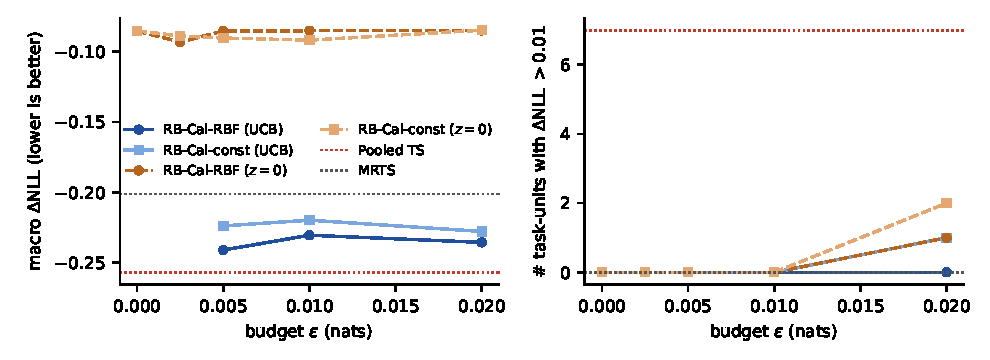
\includegraphics[width=\linewidth]{figures/eps_curve.pdf}
\caption{Effect of the budget $\varepsilon$ on the sealed split. Left: macro $\Delta$NLL; right: number of harmed task-units (of \NConfirm). Dashed lines are the pre-registered $z=0$ budgets, whose gate rejections cost most of the gain; dotted lines are pooled TS and MRTS.}
\label{fig:eps}
\end{figure}

\paragraph{Budget curve.}
Figure~\ref{fig:eps} varies $\varepsilon$.
With the UCB budget the result is insensitive to $\varepsilon$ in the tested range: RB-Cal-RBF stays between $-0.241$ and $-0.230$ with no harmed unit at any budget, while the budgeted constant and top-gap each harm one unit at $\varepsilon=0.02$.
The $z=0$ budgets stay near $-0.09$ at every $\varepsilon$ because the gate rejects them on most consensus units, and start to harm units at $\varepsilon=0.02$.
The choice $\varepsilon=0.01$ was fixed in advance to match the harm threshold, not tuned.

\paragraph{Leave-one-task-out.}
Three target tasks are few, and the case bootstrap does not reflect uncertainty over tasks.
After the confirmation run we therefore held out each of the 25 source tasks in turn, fit every method on the other 24 (training split; selection split for gates) and scored all rows of the held-out task: \NLoto{} target task-units, with CIs from resampling tasks.
The RB-Cal field configuration was kept from the selection on all 25 sources, so the held-out task took part in choosing four discrete hyperparameters; full nested reselection would have cost several hundred CPU hours (250 selections at about 1.5 hours each).
Table~\ref{tab:loto} and Figure~\ref{fig:tradeoff} show the results.
RB-Cal improves on MRTS by \LotoVsMrts{} (CI [\LotoVsMrtsLo, \LotoVsMrtsHi]; \LotoVsMrtsWin{} wins, \LotoVsMrtsLoss{} losses) and on the budgeted constant by \LotoVsConst{} (CI [\LotoVsConstLo, \LotoVsConstHi]).
It harms \LotoPrimHarm{} of \NLoto{} task-units, both barely (largest \LotoPrimHarmMax), where MRTS harms none; pooled TS, Thermometer-P and ATS-P harm \LotoPooledHarm, \LotoThermoHarm{} and \LotoAtsHarm, with worst units up to \LotoAtsWorst.
They are better on average, by \LotoVsPooled{} nats for pooled TS (CI [\LotoVsPooledLo, \LotoVsPooledHi]).

\begin{table}[t]
\centering\small
\caption{Leave-one-task-out over the 25 source tasks (\NLoto{} target task-units; \NLotoConflict{} in conflict units). Last two columns: RB-Cal-RBF minus the method, with 95\% CIs from resampling tasks, and wins/ties/losses of RB-Cal over task-units ($|\text{diff}|\le10^{-4}$ is a tie).}
\label{tab:loto}
\resizebox{\linewidth}{!}{%
\begin{tabular}{lccccccccc}
\toprule
& \multicolumn{3}{c}{All} & \multicolumn{2}{c}{Conflict} & \multicolumn{2}{c}{Consensus} & \multicolumn{2}{c}{RB-Cal $-$ method}\\
\cmidrule(lr){2-4}\cmidrule(lr){5-6}\cmidrule(lr){7-8}\cmidrule(lr){9-10}
Method & $\Delta$ & \#h & worst & $\Delta$ & \#h & $\Delta$ & \#h & diff [95\% CI] & W/T/L\\
\midrule
\inputtable{generated/tab_loto.tex}
\bottomrule
\end{tabular}}
\end{table}

\begin{figure}[t]
\centering
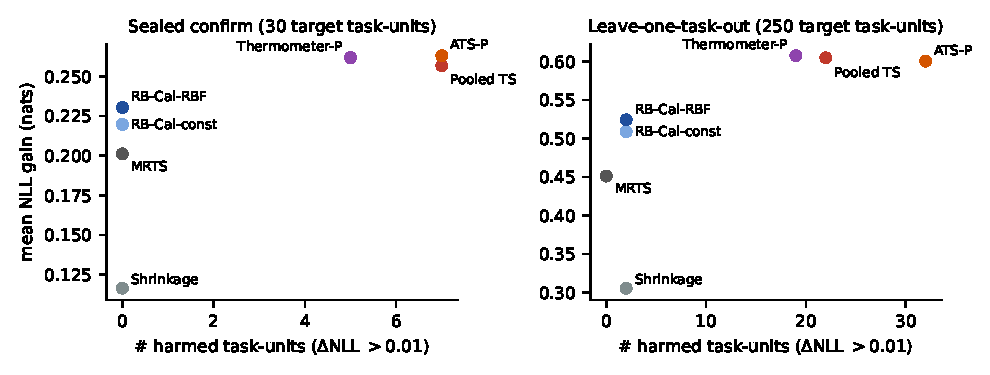
\includegraphics[width=\linewidth]{figures/tradeoff.pdf}
\caption{Mean gain against number of harmed task-units. Up and to the left is better. RB-Cal sits between the conservative MRTS and the pooled methods: most of their gain, few of their harms.}
\label{fig:tradeoff}
\end{figure}

\section{Discussion and limitations}
\paragraph{What the results support.}
On the sealed split and on \NLoto{} held-out tasks, budgeting each source's regret gives a better mean than the minimax solution and far fewer harmed tasks than pooling, and the temperature field adds a small, consistent gain over a budgeted constant.
Proposition~\ref{prop:stuck} explains when the minimax solution is inert; the regime diagnostic computed from sources alone separates units where pooling is risky (conflict: pooled methods harm 13--26 of 75 held-out task-units) from units where it is not.

\paragraph{What they do not support.}
RB-Cal does not improve average log-loss over pooled temperature scaling or the Thermometer and ATS adaptations; it trades about a tenth of the gain for safety.
It is not harm-free: two of 250 held-out task-units exceed the 0.01-nat threshold, by at most a millinat.
The UCB budget was introduced after inspecting development results; the confirmation split was untouched at that point, but the revision is not part of the pre-registration.
Before any method ran, descriptive accuracy and confidence of the raw model on the confirmation tasks were looked at once (Appendix~\ref{app:protocol}).
Thermometer-P and ATS-P are probability-feature adaptations and may be weaker than the originals, which read hidden states.
The leave-one-task-out analysis reuses hyperparameters selected with the held-out task present.

\paragraph{Scope.}
All tasks are multiple-choice with letter probabilities, the models have 7--12B parameters, there are three conflict units, and the transfer statement of Proposition~\ref{prop:transfer} only controls targets close to a mixture of the sources.
Free-form generation, larger models and formal finite-sample guarantees are outside what we tested.

\section{Conclusion}
When labelled source tasks disagree on how a model is miscalibrated, minimax calibration provably does nothing and pooled calibration harms a sizeable fraction of new tasks.
A per-source regret budget on a confidence bound sits in between: across a sealed split and a leave-one-task-out analysis on five recent models, it kept most of the pooled gain while harming far fewer target tasks.
Code, pre-registration, protocol log and all predictions will be released with the paper.

\bibliographystyle{plainnat}
\bibliography{refs}

\appendix
\section{Protocol, deviations and reproducibility}\label{app:protocol}
\paragraph{Timeline.}
(1) Source-only feasibility check: strict per-source descent (no source may get worse) was infeasible with 25 task-level sources for the conflict units.
(2) Pre-registration (written before any calibrator ran on a target).
(3) Development run with $z=0$; gate rejections on consensus units; E1 failed overall, E3 failed.
(4) Revision to the UCB budget ($z=1.645$), recorded with its reason before the confirmation split was opened.
(5) Full development run of the revision; then the code was frozen (SHA-256 prefix \texttt{b0e2f24c6e5d169d} over the calibration package and the runner) and the sealed split was scored once.
(6) Secondary analyses: Thermometer-P and ATS-P; leave-one-task-out.

\paragraph{Other deviations.}
Two HellaSwag questions share a dataset identifier; their cases were dropped on the basis of the identifier alone.
For Qwen3.5-9B with \texttt{letter\_colon} the median mass on option letters is 0.45 (0.999 with \texttt{paren}); both prompts were kept unchanged.
Once, before any calibrator was run on them, the raw accuracy and confidence of the models on the confirmation tasks were printed during a data-quality check; from then on all quality checks excluded them.
For the confirmation run, the leave-one-source-out choice of the field configuration was taken from the development run instead of being recomputed: the source files of the two phases are byte-identical (checked by SHA-256 in the runner) and the choice depends on source data only.
Re-running the development split this way reproduced every gate decision and every selected configuration; target log-probabilities were bit-identical for units fitted on the same machine and differed by at most $2.5\times10^{-8}$ for units first fitted on a different machine.

\paragraph{Compute.}
Inference: one A100 GPU, about 2.6 hours for all five models.
Calibration: CPU only, one core per unit; the full leave-one-source-out selection took 42--285 minutes per unit (three units on a laptop, seven on a cloud CPU machine with hyper-threaded cores), and a refit with a fixed configuration 6--15 minutes.

\paragraph{Released artefacts.}
Inference did not pin model revisions; every model and dataset repository used was last changed before the run, so the commits recorded afterwards are the ones used, and they are released with the code.
The five models are released under Apache-2.0; the benchmarks keep their own licences, and SciQ is restricted to non-commercial use.
Per-row probabilities for all models, the canonical splits (with the confirmation labels), the pre-registration, the dated protocol log, all fitted parameters, all target predictions with their SHA-256 hashes, and the script that generates every number, table and figure of this paper from those files.
\end{document}
